\chapter{Evaluierung}

\section{Benutzerevaluierung}
\paragraph{}
Damit es festgestellt werden könnte, ob die Anreicherung von Suchergebnissen mit aus den Snippets extrahierten Entitäten für den Benutzer auch tatsächlich hilfreich sein könnte, wurde eine Benutzerevaluierung durchgeführt. Die Evaluierung sollte folgende Fragen beantworten:

\begin{itemize}
\item Welcher Einsatz liefert dem Benutzer die zu der Anfrage am besten passende Entitäten? 
\item Wird die Geschwindigkeit der Suche durch zusätzlicher Schritt der Extraktion von Entitäten stark beeinträchtigt? Ist die Beeinträchtigung der Geschwindigkeit groß Genug, um den Benutzer bei der Suche zu stören?
\item Gibt es Korrelationen zwischen ,,standarten`` Metriken wie F-Measure und Precision/Recall und der Zufriedenheit der Benutzer, oder kann man aus der rein numerischen Metriken keine Aussage treffen, ob der Engine in der Lage ist, eine genügende Benutzerunterstützung zu leisten?
\end{itemize}

Um diese Fragen beantworten zu können, wurde eine Webseite aufgebaut, die dem Benutzer die Möglichkeit gibt, alle Engines und alle Modellen, die im Rahmen dieser Arbeit verwendet wurden, zu bewerten. Insgesamt kann der Evaluirungsvorgang in drei Schritten geteilt werden:

\begin{enumerate}
\item In dem Einleitungsschritt wird dem Benutzer erklärt, wie genau die Evaluierung abläuft, und was wir von ihm brauchen.
\item Danach muss der Benutzer alle vorhandene Kombinationen von Modellen und Engines bewerten. Dazu soll eine Frage aus der vorgegebenen Liste ausgewählt und gestellt werden, die zuerst an Bing gesendet wird, und dann an unseres Stanbol-Backend.
\item Um die Situation, wo der Benutzer sich ,,betrogen`` fühlen könnte, möglichst auszuschließen, wird dem Probanden die Möglichkeit gegeben, jede beliebige Frage zu stellen, und dann einen persönlichen schriftlichen Feedback abzugeben.
\end{enumerate}

\begin{figure}
\centering
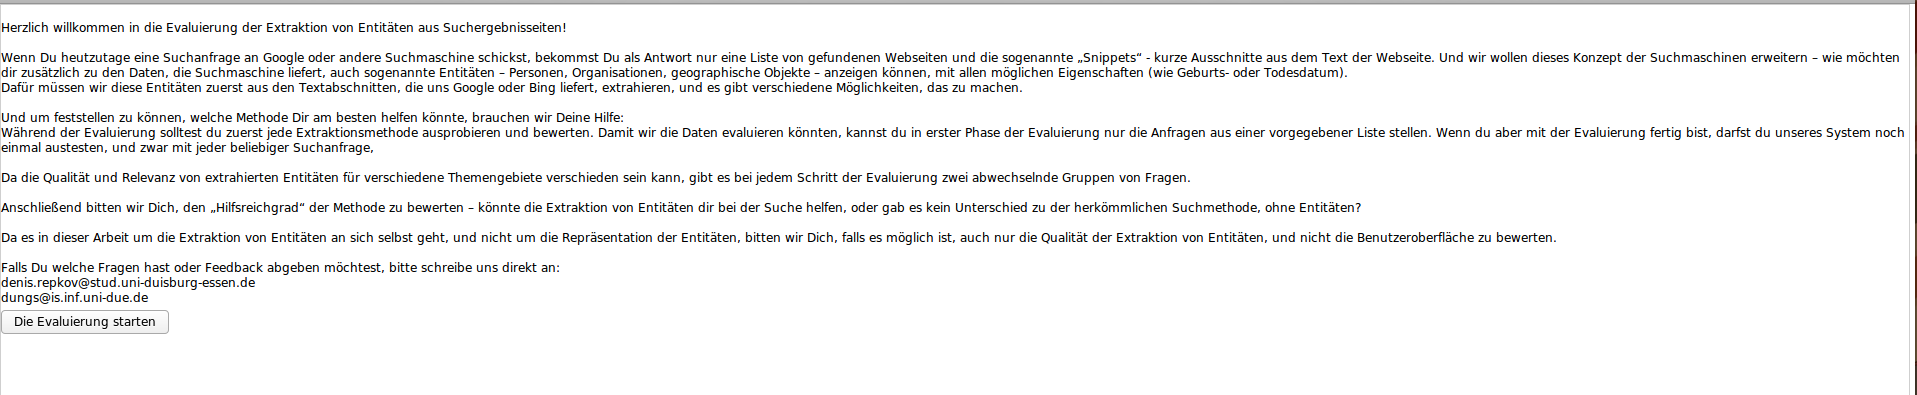
\includegraphics[width=1.0\textwidth]{Bilder/evalstep1.png}
\caption{''Einleitung in die Evaluierung''}
\label{fig:evalstep01}
\end{figure}

\begin{figure}
\centering
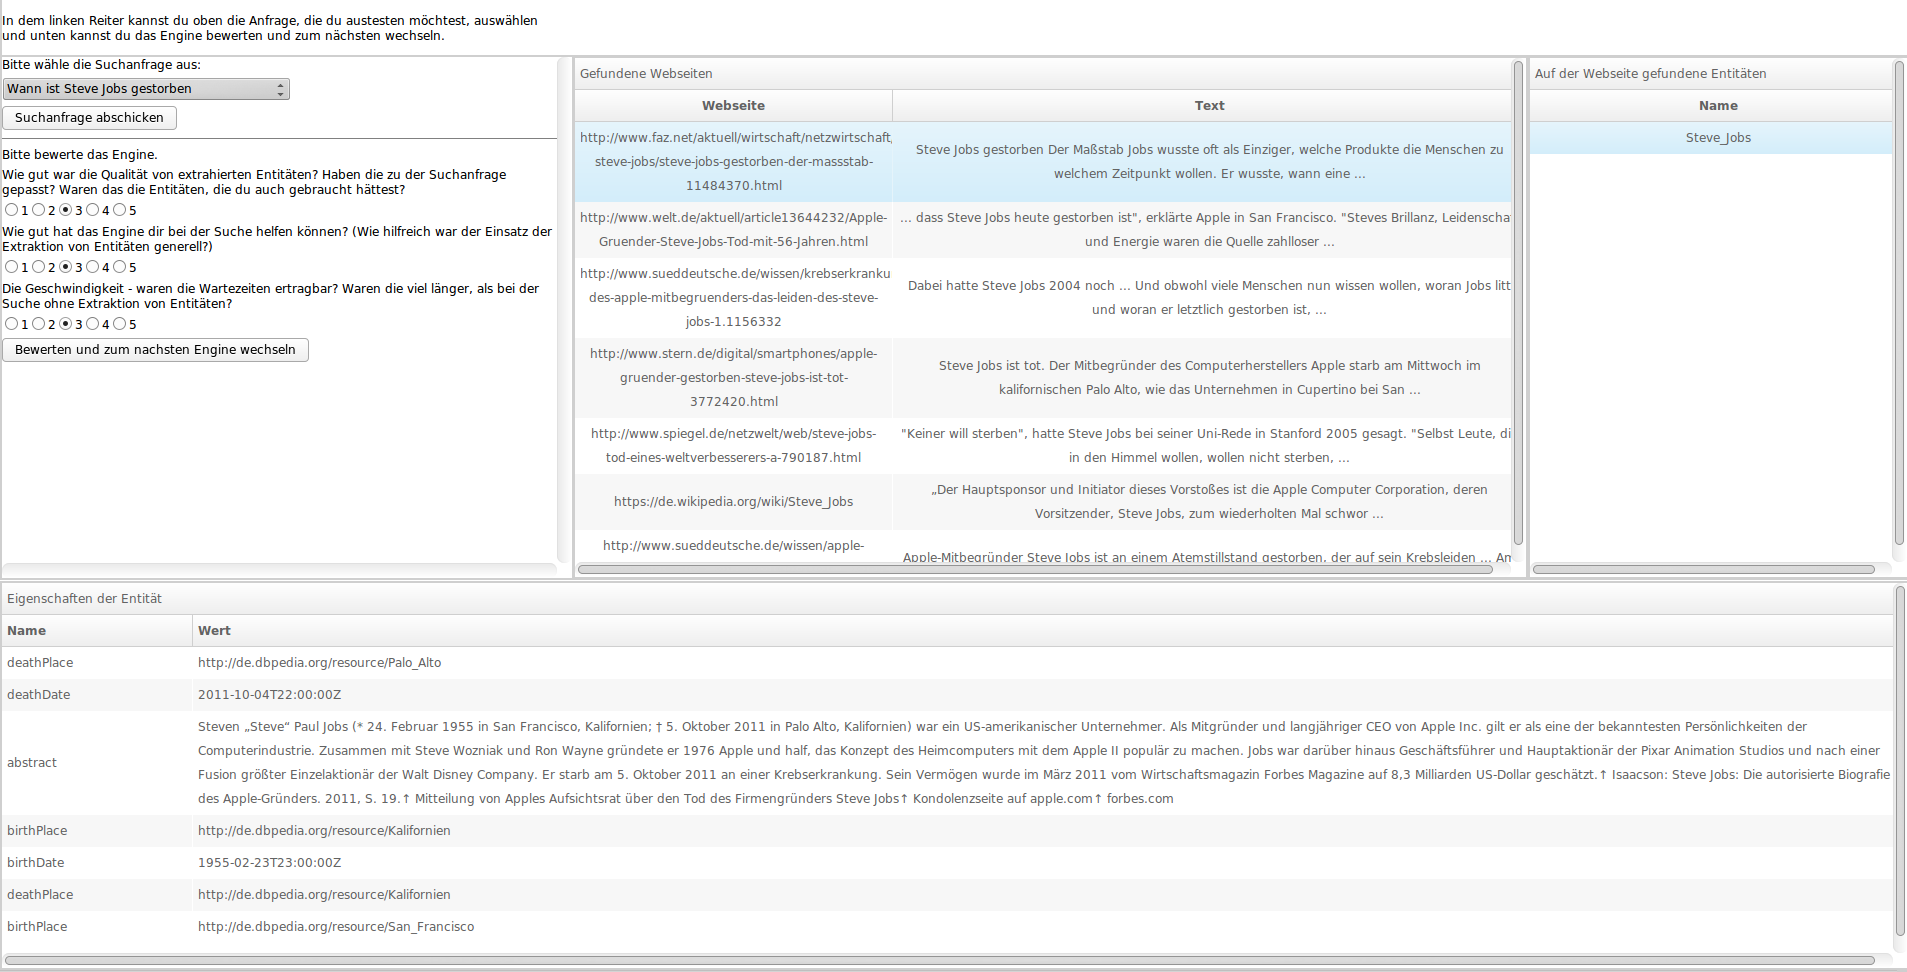
\includegraphics[width=1.0\textwidth]{Bilder/evalstep2.png}
\caption{''Bewertung eines Engines''}
\label{fig:evalstep01}
\end{figure}

\begin{figure}
\centering
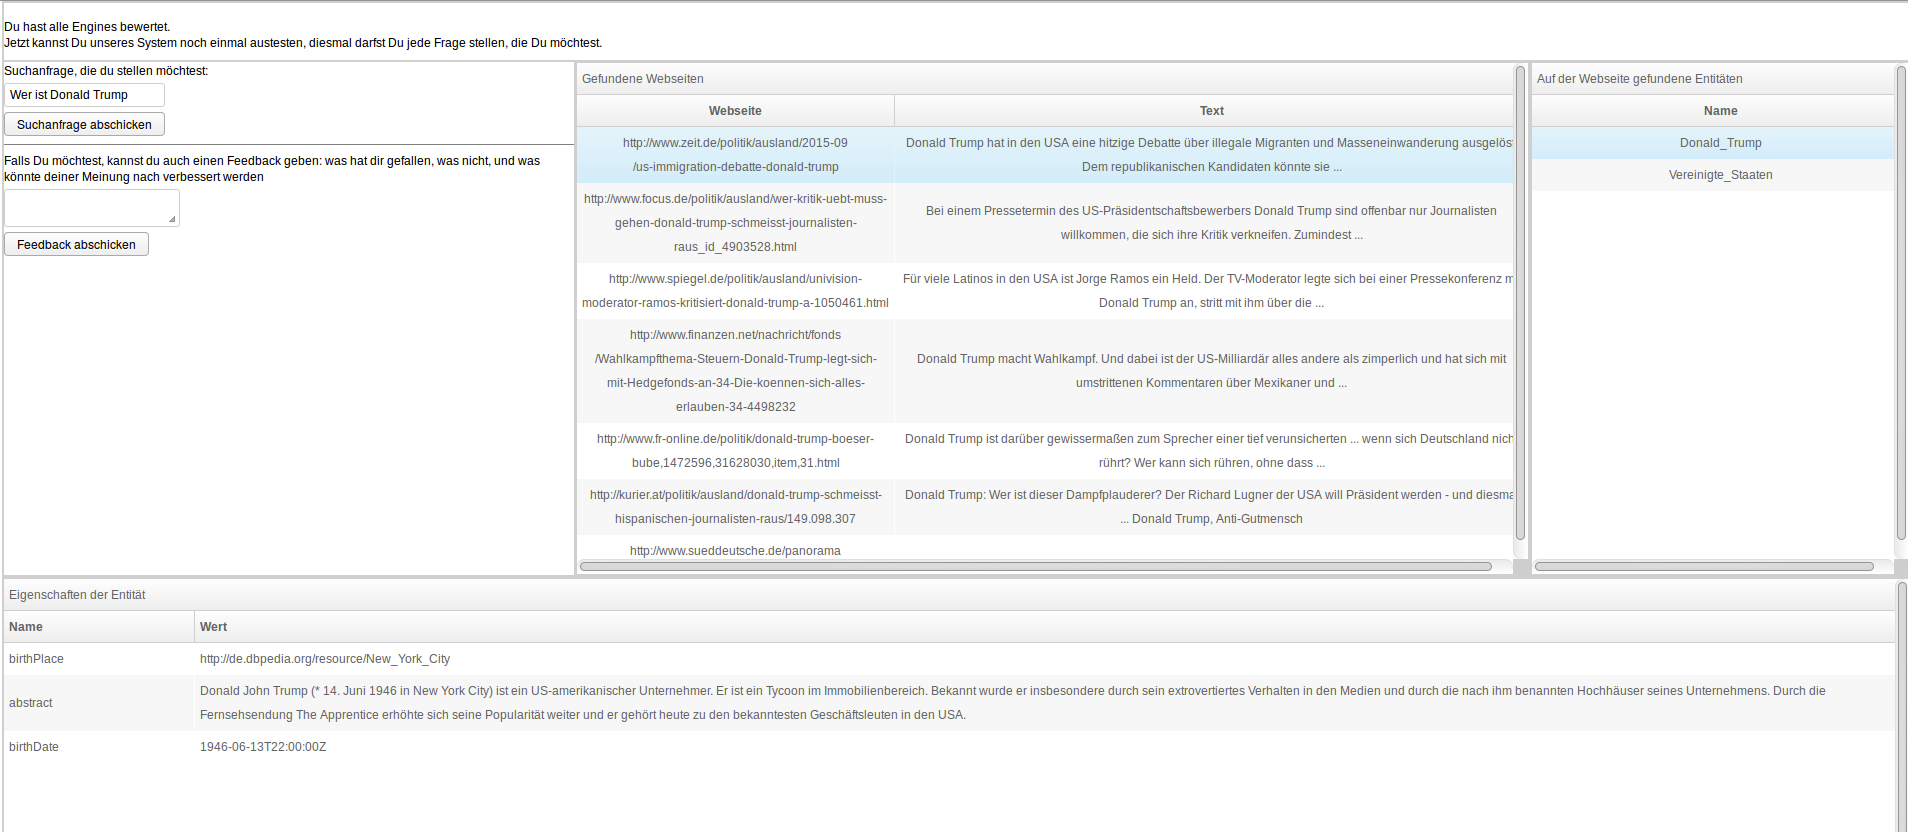
\includegraphics[width=1.0\textwidth]{Bilder/evalstep3.png}
\caption{''Der letzte Schritt der Evaluierung''}
\label{fig:evalstep01}
\end{figure}

Für jedes Engine sollen insgesamt drei Charakteristiken bewertet werden:
\begin{enumerate}
\item Qualität von extrahierten Entitäten - 
\item Geschwindigkeit der Anreicherung - 
\item ,,Hilfreichsgrad`` von dem Ansatz - 
\end{enumerate}

\section{Zusammenfassung}
Erkenntnissen aus der Studie und den Konsequenzen für die Arbeit.